\documentclass[10pt]{article}
\usepackage{soul}
\usepackage{mathtools}
\DeclarePairedDelimiter{\ceil}{\lceil}{\rceil}
\usepackage{graphicx}
\usepackage{float}
\usepackage{amsmath}
\usepackage{amssymb}
\usepackage{listings}
\usepackage{hyperref}
\usepackage[margin=1in]{geometry}
\usepackage{xcolor}
\usepackage{booktabs}
\usepackage{array}
\usepackage{tikz}
\usetikzlibrary{arrows.meta, decorations.pathreplacing, calc}

\definecolor{codegreen}{rgb}{0,0.6,0}
\definecolor{codegray}{rgb}{0.5,0.5,0.5}
\definecolor{codepurple}{rgb}{0.58,0,0.82}
\definecolor{backcolour}{rgb}{0.9,0.9,0.95}
\definecolor{bluelight}{rgb}{0.78,0.88,1.0}
\definecolor{greenlight}{rgb}{0.78,1.0,0.82}
\definecolor{redlight}{rgb}{1.0,0.78,0.78}
\definecolor{orangelight}{rgb}{1.0,0.88,0.65}

\title{\texttt{get\_log\_probs} --- Step-by-Step Explanation}
\author{JR}
\date{\today}

\lstdefinestyle{mystyle}{
    commentstyle=\color{codegreen},
    keywordstyle=\color{magenta},
    numberstyle=\tiny\color{codegray},
    stringstyle=\color{codepurple},
    basicstyle=\ttfamily\footnotesize,
    breakatwhitespace=false,
    breaklines=true,
    captionpos=b,
    keepspaces=true,
    numbers=left,
    numbersep=5pt,
    showspaces=false,
    showstringspaces=false,
    showtabs=false,
    tabsize=2
}
\lstset{language=Python}
\lstset{style=mystyle}

\providecommand{\tightlist}{%
  \setlength{\itemsep}{0pt}\setlength{\parskip}{0pt}}

\begin{document}

\maketitle
\tableofcontents
\newpage

% =============================================
\section{Overview}
% =============================================

\texttt{get\_log\_probs} is a utility function used during transformer training.
Given the model's raw output (logits) and the actual token sequence, it returns
the \textbf{log probability the model assigned to each correct next token}.

\begin{lstlisting}
def get_log_probs(
    logits: Float[Tensor, "batch posn d_vocab"],
    tokens: Int[Tensor, "batch posn"]
) -> Float[Tensor, "batch posn-1"]:
    log_probs = logits.log_softmax(dim=-1)
    log_probs_for_tokens = (
        log_probs[:, :-1]
            .gather(dim=-1, index=tokens[:, 1:].unsqueeze(-1))
            .squeeze(-1)
    )
    return log_probs_for_tokens
\end{lstlisting}

% =============================================
\section{Inputs and Output}
% =============================================

\begin{center}
\begin{tabular}{lll}
\toprule
\textbf{Argument} & \textbf{Shape} & \textbf{Meaning} \\
\midrule
\texttt{logits} & $[\text{batch},\ \text{posn},\ d_\text{vocab}]$ & Raw unnormalized scores for every vocab token at every position \\
\texttt{tokens} & $[\text{batch},\ \text{posn}]$ & Actual token IDs in the sequence \\
\midrule
\textit{return} & $[\text{batch},\ \text{posn}-1]$ & Log prob of the correct next token at each position \\
\bottomrule
\end{tabular}
\end{center}

% =============================================
\section{The Core Alignment Idea}
% =============================================

A transformer at position $i$ predicts the token at position $i+1$.
This means the model's output at position $i$ must be evaluated against
the \emph{next} token in the sequence, not the current one.

\medskip
\noindent Consider the sequence \texttt{["The", "cat", "sat", "."]} with token IDs $[1, 2, 3, 4]$:

\begin{center}
\begin{tabular}{ccccc}
\toprule
Position & 0 & 1 & 2 & 3 \\
Token & \texttt{"The"} & \texttt{"cat"} & \texttt{"sat"} & \texttt{"."} \\
\midrule
Model predicts $\to$ & \texttt{"cat"} & \texttt{"sat"} & \texttt{"."} & \textit{(no target)} \\
\bottomrule
\end{tabular}
\end{center}

\medskip
The last position has no ground-truth next token to score against, so the output
has shape $\text{posn} - 1$ rather than $\text{posn}$.

% =============================================
\section{How the Two Slices Work}
% =============================================

\subsection{\texttt{log\_probs[:, :-1]} --- Slicing a Three-Dimensional Tensor}

\texttt{log\_probs} has shape $[\text{batch},\ \text{posn},\ d_\text{vocab}]$
--- three axes.
The notation \texttt{[:, :-1]} supplies only \textbf{two} explicit index
expressions. Python and PyTorch apply a simple rule:

\begin{quote}
\textit{Any trailing dimension not mentioned in the index expression receives
an implicit \texttt{:} --- meaning ``keep every element along that axis''.}
\end{quote}

\noindent Therefore \texttt{log\_probs[:, :-1]} is \emph{exactly} equivalent
to \texttt{log\_probs[:, :-1, :]}. The three index slots map to axes as follows:

\begin{center}
\begin{tabular}{clll}
\toprule
\textbf{Slot} & \textbf{Value} & \textbf{Axis} & \textbf{Effect} \\
\midrule
1st & \texttt{:}          & dim 0 --- batch       & Keep every batch item (unchanged) \\
2nd & \texttt{:-1}        & dim 1 --- posn        & Keep indices $0, 1, \ldots, \text{posn}-2$;
                                                     \emph{drop} the last position \\
3rd & \texttt{:} (implicit) & dim 2 --- $d_\text{vocab}$ & Keep \emph{every} vocabulary entry (unchanged) \\
\bottomrule
\end{tabular}
\end{center}

\medskip\noindent
\textbf{Shape: $[\text{batch},\ \text{posn},\ d_\text{vocab}]$
$\;\longrightarrow\;$ $[\text{batch},\ \text{posn}-1,\ d_\text{vocab}]$}

\medskip\noindent
The critical insight is that the third dimension is \textbf{entirely
untouched}. The slice only removes one ``slice of pages'' along the position
axis. For every surviving (batch, posn) pair the full $d_\text{vocab}$-wide
row of log probabilities is preserved intact. Visualise
\texttt{log\_probs} as a stack of $\text{batch}$ matrices, each of size
$\text{posn} \times d_\text{vocab}$. The operation removes the \emph{last
row} from every matrix while leaving each row's full width untouched:

\begin{figure}[H]
\centering
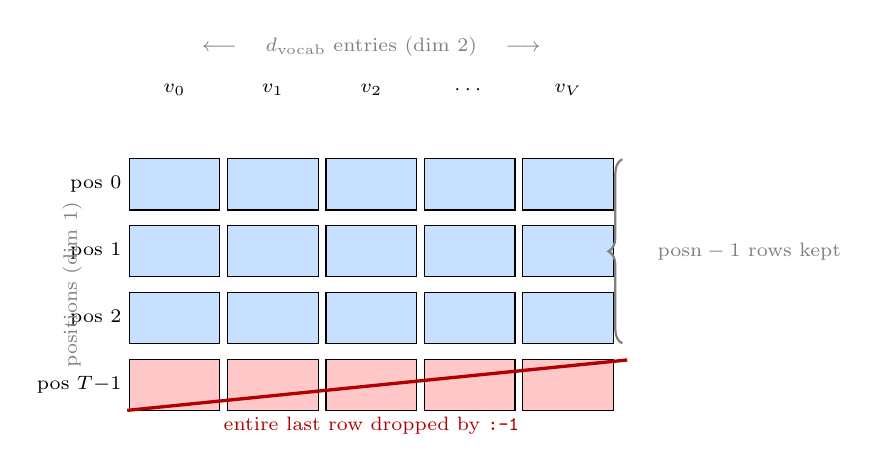
\begin{tikzpicture}[
  kept/.style={draw, minimum width=1.15cm, minimum height=0.65cm,
               align=center, font=\ttfamily\scriptsize, fill=bluelight},
  drop/.style={draw, minimum width=1.15cm, minimum height=0.65cm,
               align=center, font=\ttfamily\scriptsize,
               fill=redlight, text=gray},
  lbl/.style={font=\scriptsize\bfseries},
]
%% Column headers (vocab dimension)
\foreach \c/\v in {0/$v_0$, 1/$v_1$, 2/$v_2$, 3/$\cdots$, 4/$v_{V}$}{
  \node[lbl] at (\c*1.25, 4.3) {\v};
}
\node[font=\scriptsize, gray] at (2*1.25, 4.85)
  {$\longleftarrow\quad d_\text{vocab}\text{ entries (dim 2)}\quad\longrightarrow$};

%% Kept rows (positions 0 … posn-2)
\foreach \r/\rl in {0/pos 0, 1/pos 1, 2/pos 2}{
  \node[font=\scriptsize, anchor=east] at (-0.55, 3.1-\r*0.85) {\rl};
  \foreach \c in {0,1,2,3,4}{
    \node[kept] at (\c*1.25, 3.1-\r*0.85) {};
  }
}

%% Dropped row (last position)
\node[font=\scriptsize, anchor=east] at (-0.55, 3.1-3*0.85) {pos $T{-}1$};
\foreach \c in {0,1,2,3,4}{
  \node[drop] at (\c*1.25, 3.1-3*0.85) {};
}
\draw[red!70!black, very thick]
  (-0.6, 3.1-3*0.85-0.32) -- (4.6*1.25, 3.1-3*0.85+0.32);
\node[font=\scriptsize, red!70!black] at (2*1.25, 3.1-3*0.85-0.52)
  {entire last row dropped by \texttt{:-1}};

%% Right brace: kept rows
\draw[decorate, decoration={brace, amplitude=5pt, mirror}, thick, gray]
  ($(4.55*1.25, 3.1+0.32)$) -- ($(4.55*1.25, 3.1-2*0.85-0.32)$)
  node[midway, right=9pt, font=\scriptsize, gray]
    {$\text{posn}-1$ rows kept};

%% y-axis label
\node[font=\scriptsize, gray, rotate=90] at (-1.3, 3.1-1.5*0.85)
  {positions (dim 1)};
\end{tikzpicture}
\caption{Effect of \texttt{log\_probs[:, :-1]} on one batch item.
The slice operates \emph{only} on dim 1 (position axis):
it discards the last row (pos $T{-}1$, red).
The entire width of dim 2 --- all $d_\text{vocab}$ log-probability
entries --- is preserved for every kept row (blue).
Dim 0 (batch) is also untouched; the same operation applies identically
to every item in the batch.}
\end{figure}

% - - - - - - - - - - - - - - - - - - - - - -
\subsection{\texttt{tokens[:, 1:]} --- Slicing a Two-Dimensional Tensor}
% - - - - - - - - - - - - - - - - - - - - - -

\texttt{tokens} has shape $[\text{batch},\ \text{posn}]$ --- two axes.
The slice \texttt{[:, 1:]} maps to:

\begin{center}
\begin{tabular}{clll}
\toprule
\textbf{Slot} & \textbf{Value} & \textbf{Axis} & \textbf{Effect} \\
\midrule
1st & \texttt{:}  & dim 0 --- batch & Keep every batch item \\
2nd & \texttt{1:} & dim 1 --- posn  & Keep indices $1, 2, \ldots, \text{posn}-1$;
                                      \emph{drop} index 0 (the first token) \\
\bottomrule
\end{tabular}
\end{center}

\medskip\noindent
\textbf{Shape: $[\text{batch},\ \text{posn}]$
$\;\longrightarrow\;$ $[\text{batch},\ \text{posn}-1]$}

\medskip\noindent
The slice expression \texttt{1:} is standard Python \emph{start-from-1-to-end}
notation. In general \texttt{a:b} selects elements whose indices satisfy
$a \le i < b$; omitting the upper bound means ``go all the way to the end''.
So \texttt{1:} retains every index $\ge 1$, dropping only index 0.

\medskip\noindent
The semantic effect is a \textbf{left-shift by one position}: element $i$ in
the result is the element that was at position $i+1$ in the original tensor.
Concretely, for the sequence
$[\texttt{"The"},\ \texttt{"cat"},\ \texttt{"sat"},\ \texttt{"."}]$
with token IDs $[1, 2, 3, 4]$:

\begin{center}
\begin{tabular}{lcccc}
\toprule
 & \multicolumn{4}{c}{\textbf{Position in dim 1}} \\
 & 0 & 1 & 2 & 3 \\
\midrule
\textbf{Before} \texttt{tokens} &
  \texttt{"The"} (1) & \texttt{"cat"} (2) & \texttt{"sat"} (3) & \texttt{"."} (4) \\
\midrule
\textbf{After} \texttt{tokens[:,\,1:]} &
  \textcolor{gray}{dropped} & $\underbrace{\texttt{"cat"}}_{\to\text{index }0}$ (2) &
  $\underbrace{\texttt{"sat"}}_{\to\text{index }1}$ (3) &
  $\underbrace{\texttt{"."}}_{\to\text{index }2}$ (4) \\
\bottomrule
\end{tabular}
\end{center}

\medskip\noindent
The first token \texttt{"The"} is dropped because it is the starting token
--- no earlier model output exists that should have predicted it as a
\emph{next} token. What remains is the list of \textbf{ground-truth targets}:
exactly the token each position $0, 1, \ldots, \text{posn}-2$ was supposed
to predict.

\medskip\noindent
\textbf{Why the shapes now match.}
After both slices:

\[
  \underbrace{\texttt{log\_probs[:, :-1]}}_{\text{shape }[\text{batch},\,\text{posn}-1,\,d_\text{vocab}]}
  \quad\text{and}\quad
  \underbrace{\texttt{tokens[:, 1:]}}_{\text{shape }[\text{batch},\,\text{posn}-1]}
\]

Both have the same $[\text{batch},\ \text{posn}-1]$ prefix.
Position $i$ in \texttt{log\_probs[:, :-1]} holds the distribution the
model produced at position $i$, and position $i$ in \texttt{tokens[:, 1:]}
holds the correct token the model should have predicted at that
position --- namely the token originally at position $i+1$.

% =============================================
\section{Diagram 1 --- Sequence Alignment and Slicing}
% =============================================

The two slicing operations (\texttt{log\_probs[:,~:-1]} and \texttt{tokens[:,~1:]})
create a matched pair of tensors: every prediction position lines up with its
ground-truth target. \textcolor{red!60!black}{Red} cells are discarded;
\textcolor{blue!60!black}{blue} cells are prediction blocks;
\textcolor{green!50!black}{green} cells are target tokens.

\begin{figure}[H]
\centering
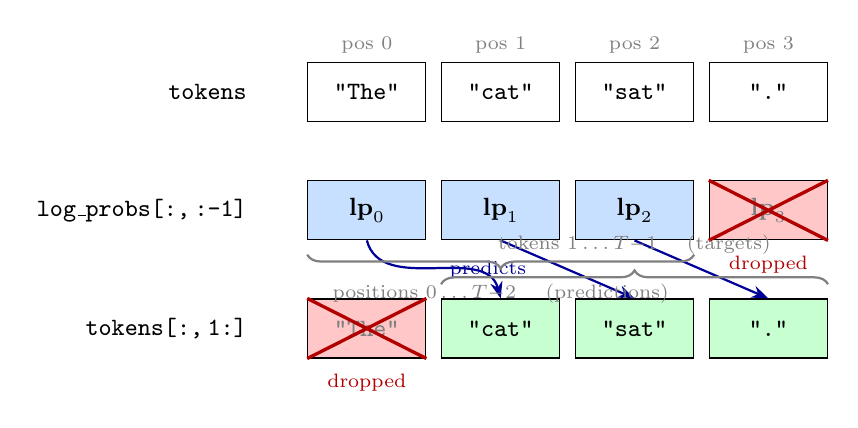
\begin{tikzpicture}[
  tok/.style={
    draw, minimum width=1.5cm, minimum height=0.75cm,
    align=center, font=\ttfamily\small
  },
  pred/.style={
    draw, minimum width=1.5cm, minimum height=0.75cm,
    align=center, font=\ttfamily\small, fill=bluelight
  },
  tgt/.style={
    draw, minimum width=1.5cm, minimum height=0.75cm,
    align=center, font=\ttfamily\small, fill=greenlight
  },
  drop/.style={
    draw, minimum width=1.5cm, minimum height=0.75cm,
    align=center, font=\ttfamily\small, fill=redlight, text=gray
  },
  lbl/.style={font=\small\bfseries, anchor=east},
  arr/.style={-{Stealth[length=6pt]}, thick, blue!60!black},
]

%% ---- Full token sequence (y = 3.0) ----
\node[lbl] at (-1.4, 3.0) {\texttt{tokens}};
\node[tok] at (0*1.7, 3.0) {"The"};
\node[tok] at (1*1.7, 3.0) {"cat"};
\node[tok] at (2*1.7, 3.0) {"sat"};
\node[tok] at (3*1.7, 3.0) {"."};
\foreach \x/\p in {0/0, 1/1, 2/2, 3/3}{
  \node[font=\scriptsize, gray] at (\x*1.7, 3.6) {pos \p};
}

%% ---- log_probs[:, :-1]  (y = 1.5) ----
\node[lbl] at (-1.4, 1.5) {\texttt{log\_probs[:,\,:-1]}};
\node[pred] (lp0) at (0*1.7, 1.5) {$\mathbf{lp}_0$};
\node[pred] (lp1) at (1*1.7, 1.5) {$\mathbf{lp}_1$};
\node[pred] (lp2) at (2*1.7, 1.5) {$\mathbf{lp}_2$};
\node[drop] (lp3) at (3*1.7, 1.5) {$\mathbf{lp}_3$};
\draw[red!70!black, very thick]
  (lp3.north west) -- (lp3.south east)
  (lp3.north east) -- (lp3.south west);
\node[font=\scriptsize, red!70!black, below=2pt] at (lp3.south) {dropped};

%% ---- tokens[:, 1:]  (y = 0.0) ----
\node[lbl] at (-1.4, 0.0) {\texttt{tokens[:,\,1:]}};
\node[drop] (tk0) at (0*1.7, 0.0) {"The"};
\node[tgt]  (tk1) at (1*1.7, 0.0) {"cat"};
\node[tgt]  (tk2) at (2*1.7, 0.0) {"sat"};
\node[tgt]  (tk3) at (3*1.7, 0.0) {"."};
\draw[red!70!black, very thick]
  (tk0.north west) -- (tk0.south east)
  (tk0.north east) -- (tk0.south west);
\node[font=\scriptsize, red!70!black, below=2pt] at (tk0.south) {dropped};

%% ---- Alignment arrows ----
\draw[arr] (lp0.south) to[out=-75, in=105]
  node[midway, right=2pt, font=\scriptsize] {predicts} (tk1.north);
\draw[arr] (lp1.south) -- (tk2.north);
\draw[arr] (lp2.south) -- (tk3.north);

%% ---- Braces ----
\draw[decorate, decoration={brace, amplitude=5pt, mirror}, thick, gray]
  ($(lp0.south west)+(0,-0.18)$) -- ($(lp2.south east)+(0,-0.18)$)
  node[midway, below=7pt, font=\scriptsize, gray]
    {positions $0\ldots T{-}2$ \quad (predictions)};

\draw[decorate, decoration={brace, amplitude=5pt}, thick, gray]
  ($(tk1.north west)+(0,0.18)$) -- ($(tk3.north east)+(0,0.18)$)
  node[midway, above=7pt, font=\scriptsize, gray]
    {tokens $1\ldots T{-}1$ \quad (targets)};

\end{tikzpicture}
\caption{Slicing alignment. Each blue prediction block $\mathbf{lp}_i$ is
evaluated against the green target token at position $i{+}1$.
The red cells (last prediction, first token) are discarded because they have
no counterpart.}
\end{figure}

% =============================================
\section{Diagram 2 --- The \texttt{gather} Operation}
% =============================================

After slicing, \texttt{log\_probs[:,~:-1]} is a matrix of shape
$[\text{posn}{-}1,\ d_\text{vocab}]$.
\texttt{gather} selects \textbf{one cell per row} --- the log probability of
the actual next token --- and assembles them into the output vector.

\begin{figure}[H]
\centering
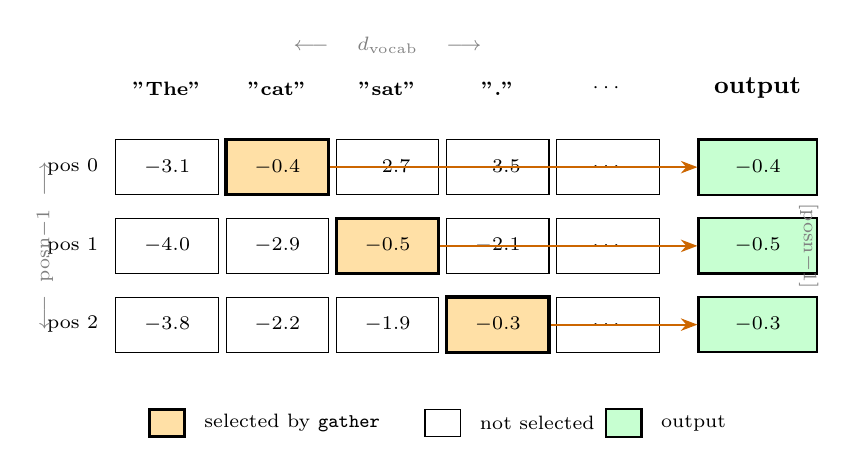
\begin{tikzpicture}[
  cell/.style={
    draw, minimum width=1.3cm, minimum height=0.7cm,
    align=center, font=\ttfamily\scriptsize
  },
  hi/.style={
    draw, minimum width=1.3cm, minimum height=0.7cm,
    align=center, font=\ttfamily\scriptsize\bfseries,
    fill=orangelight, very thick
  },
  outvec/.style={
    draw, minimum width=1.5cm, minimum height=0.7cm,
    align=center, font=\ttfamily\scriptsize\bfseries,
    fill=greenlight, thick
  },
  arr/.style={-{Stealth[length=6pt]}, thick, orange!80!black},
]

%% ---- Vocab column headers ----
\node[font=\scriptsize\bfseries] at (0*1.4, 4.0) {"The"};
\node[font=\scriptsize\bfseries] at (1*1.4, 4.0) {"cat"};
\node[font=\scriptsize\bfseries] at (2*1.4, 4.0) {"sat"};
\node[font=\scriptsize\bfseries] at (3*1.4, 4.0) {"."};
\node[font=\scriptsize\bfseries] at (4*1.4, 4.0) {$\cdots$};
\node[font=\scriptsize, gray] at (2*1.4, 4.55)
  {$\longleftarrow\quad d_\text{vocab} \quad\longrightarrow$};

%% ---- Row 0: pos 0 predicts "cat" (col 1) ----
\node[font=\scriptsize, anchor=east] at (-0.75, 3.0) {pos 0};
\node[cell]          at (0*1.4, 3.0) {$-3.1$};
\node[hi]  (r0hi)    at (1*1.4, 3.0) {$-0.4$};
\node[cell]          at (2*1.4, 3.0) {$-2.7$};
\node[cell]          at (3*1.4, 3.0) {$-3.5$};
\node[cell]          at (4*1.4, 3.0) {$\cdots$};

%% ---- Row 1: pos 1 predicts "sat" (col 2) ----
\node[font=\scriptsize, anchor=east] at (-0.75, 2.0) {pos 1};
\node[cell]          at (0*1.4, 2.0) {$-4.0$};
\node[cell]          at (1*1.4, 2.0) {$-2.9$};
\node[hi]  (r1hi)    at (2*1.4, 2.0) {$-0.5$};
\node[cell]          at (3*1.4, 2.0) {$-2.1$};
\node[cell]          at (4*1.4, 2.0) {$\cdots$};

%% ---- Row 2: pos 2 predicts "." (col 3) ----
\node[font=\scriptsize, anchor=east] at (-0.75, 1.0) {pos 2};
\node[cell]          at (0*1.4, 1.0) {$-3.8$};
\node[cell]          at (1*1.4, 1.0) {$-2.2$};
\node[cell]          at (2*1.4, 1.0) {$-1.9$};
\node[hi]  (r2hi)    at (3*1.4, 1.0) {$-0.3$};
\node[cell]          at (4*1.4, 1.0) {$\cdots$};

%% Axis label
\node[font=\scriptsize, gray, rotate=90] at (-1.55, 2.0)
  {$\longleftarrow\;\text{posn}{-}1\;\longrightarrow$};

%% ---- Output vector ----
\node[font=\small\bfseries] at (7.5, 4.0) {output};
\node[outvec] (o0) at (7.5, 3.0) {$-0.4$};
\node[outvec] (o1) at (7.5, 2.0) {$-0.5$};
\node[outvec] (o2) at (7.5, 1.0) {$-0.3$};
\node[font=\scriptsize, gray, rotate=-90] at (8.15, 2.0)
  {$[\text{posn}{-}1]$};

%% ---- Gather arrows ----
\draw[arr] (r0hi.east) to[out=0, in=180] (o0.west);
\draw[arr] (r1hi.east) to[out=0, in=180] (o1.west);
\draw[arr] (r2hi.east) to[out=0, in=180] (o2.west);

%% ---- Legend ----
\node[hi,     minimum width=0.45cm, minimum height=0.35cm] at (0.0,  -0.25) {};
\node[font=\scriptsize, anchor=west] at (0.35, -0.25) {selected by \texttt{gather}};
\node[cell,   minimum width=0.45cm, minimum height=0.35cm] at (3.5,  -0.25) {};
\node[font=\scriptsize, anchor=west] at (3.85, -0.25) {not selected};
\node[outvec, minimum width=0.45cm, minimum height=0.35cm] at (5.8,  -0.25) {};
\node[font=\scriptsize, anchor=west] at (6.15, -0.25) {output};

\end{tikzpicture}
\caption{The \texttt{gather} operation. Each row of
\texttt{log\_probs[:,\,:-1]} holds log probabilities over all $d_\text{vocab}$
tokens. \texttt{gather} picks the \textbf{highlighted} (orange) cell ---
the log prob of the true next token --- and writes it to the output vector.
The final \texttt{squeeze(-1)} collapses the trailing size-1 dimension,
yielding shape $[\text{batch},\,\text{posn}{-}1]$.}
\end{figure}

% =============================================
\section{Step-by-Step Walkthrough}
% =============================================

\subsection{Step 1 --- Convert logits to log probabilities}

\begin{lstlisting}
log_probs = logits.log_softmax(dim=-1)
# shape: [batch, posn, d_vocab]  (unchanged)
\end{lstlisting}

\texttt{log\_softmax} is applied along \texttt{dim=-1} (the vocab dimension).
For each position $p$ in batch item $b$, it computes:

\[
  \text{log\_probs}[b, p, v] = \log \frac{e^{\text{logits}[b,p,v]}}{\sum_{v'} e^{\text{logits}[b,p,v']}}
  = \log P(\text{token}_v \mid \text{context up to } p)
\]

Using \texttt{log\_softmax} instead of \texttt{softmax + log} is numerically
stable because it avoids computing very small probabilities before taking the log.

\subsection{Step 2 --- Drop the last position}

\begin{lstlisting}
log_probs[:, :-1]
# shape: [batch, posn-1, d_vocab]
\end{lstlisting}

The model at the last position has no next token to be evaluated against,
so we discard it. Only positions $0, 1, \ldots, \text{posn}-2$ remain.

\subsection{Step 3 --- Get the actual next tokens}

\begin{lstlisting}
tokens[:, 1:]
# shape: [batch, posn-1]
\end{lstlisting}

We drop the first token and keep the rest. These are the ground-truth
\emph{targets}: the token at index $1$ is what position $0$ should have
predicted, the token at index $2$ is what position $1$ should have predicted,
and so on.

\medskip
\noindent The alignment is now:

\[
  \underbrace{\text{log\_probs}[:, :-1]}_{\text{predictions from positions } 0 \ldots \text{posn}-2}
  \quad \longleftrightarrow \quad
  \underbrace{\text{tokens}[:, 1:]}_{\text{targets at positions } 1 \ldots \text{posn}-1}
\]

\subsection{Step 4 --- Add a trailing dimension for \texttt{gather}}

\begin{lstlisting}
tokens[:, 1:].unsqueeze(-1)
# shape: [batch, posn-1, 1]
\end{lstlisting}

\texttt{torch.gather} requires the \emph{index} tensor to have the same number
of dimensions as the \emph{source} tensor.
The source \texttt{log\_probs[:, :-1]} has 3 dimensions
$[\text{batch}, \text{posn}-1, d_\text{vocab}]$, so we add a trailing
dimension of size 1 to the index tensor.

\subsection{Step 5 --- Select the log prob for the correct token}

\begin{lstlisting}
log_probs[:, :-1].gather(dim=-1, index=tokens[:, 1:].unsqueeze(-1))
# shape: [batch, posn-1, 1]
\end{lstlisting}

\texttt{gather(dim=-1, index=idx)} picks, for each $(b, p)$ slot, exactly one
value along the vocab dimension:

\[
  \text{output}[b, p, 0]
  = \text{log\_probs}[b,\ p,\ \underbrace{\text{tokens}[b,\ p+1]}_{\text{true next token ID}}]
  = \log P(\text{true next token} \mid \text{context})
\]

\subsection{Step 6 --- Remove the trailing size-1 dimension}

\begin{lstlisting}
.squeeze(-1)
# shape: [batch, posn-1]
\end{lstlisting}

\texttt{squeeze(-1)} removes the trailing dimension of size 1 introduced
by \texttt{unsqueeze} and \texttt{gather}, giving the clean output shape.

% =============================================
\section{Concrete Example}
% =============================================

Let batch $= 1$, sequence $= [\texttt{"The"}, \texttt{"cat"}, \texttt{"sat"}]$,
token IDs $= [1, 2, 3]$.

\begin{center}
\begin{tabular}{ll}
\toprule
\textbf{Tensor} & \textbf{What it contains} \\
\midrule
\texttt{log\_probs} & shape $[1, 3, d_\text{vocab}]$; log probs at all 3 positions \\
\texttt{log\_probs[:, :-1]} & shape $[1, 2, d_\text{vocab}]$; positions 0 and 1 only \\
\texttt{tokens[:, 1:]} & $[[2, 3]]$; ``cat'' and ``sat'' are the targets \\
\texttt{gather} output & picks \texttt{log\_probs[0,0,2]} and \texttt{log\_probs[0,1,3]} \\
\midrule
\textit{result} & $\bigl[\log P(\texttt{"cat"} \mid \texttt{"The"}),\;
                         \log P(\texttt{"sat"} \mid \texttt{"The cat"})\bigr]$ \\
\bottomrule
\end{tabular}
\end{center}

% =============================================
\section{Why Log Probabilities?}
% =============================================

\begin{itemize}
  \item \textbf{Numerical stability.} Raw probabilities of long sequences
        become vanishingly small; working in log space avoids underflow.

  \item \textbf{Summability.} The log probability of an entire sequence
        factorises as a sum:
        \[
          \log P(x_1, x_2, \ldots, x_T) = \sum_{t=1}^{T} \log P(x_t \mid x_{<t})
        \]

  \item \textbf{Direct connection to cross-entropy loss.}
        Averaging the negated log probs over the sequence gives the
        standard language-modelling cross-entropy loss:
        \[
          \mathcal{L} = -\frac{1}{T-1} \sum_{t=0}^{T-2}
          \log P(x_{t+1} \mid x_{\leq t})
        \]
\end{itemize}

\end{document}
